%        File: 03140299.tex
%     Created: Sun Feb 15 04:00 AM 2015 J
% Last Change: Sun Feb 15 04:00 AM 2015 J
%
\documentclass[a4paper,10pt,twocolumn]{jarticle}

% to input Japanese
\usepackage[japanese]{babel}

% for itemize[noitemsep] (compact itemizing)
\usepackage{enumitem}

% to be standard a4paper
\usepackage{geometry}
\geometry{left=20mm, right=20mm, top=20mm, bottom=40mm}

% to insert figures
\usepackage[dvipdfmx]{graphicx}

%% to insert source codes
% \usepackage{listings, jlisting}
% \renewcommand{\lstlistingname}{list}
% \lstset{language=C,
%   basicstyle=\ttfamily\scriptsize,
%   commentstyle=\textit,
%   classoffset=1,
%   keywordstyle=\bfseries,
%   frame=tRBl,
%   framesep=5pt,
%   showstringspaces=false,
%   numbers=left,
%   stepnumber=1,
%   numberstyle=\tiny,
%   tabsize=2
% }

%%%%%%%%%%%%%%%%%%
% title & author %
%%%%%%%%%%%%%%%%%%
\title{自主プロジェクトレポート \\ keyopener - 鍵の遠隔操作システム}
\author{03-140299 東京大学機械情報工学科 3年 和田健太郎}





\begin{document}





\maketitle





\section{概要}
近年スマートフォンなどのネットワークに常時接続される
デバイスの増加に伴い, あらゆるモノがオンライン化する
「モノのインターネット」 (IoT = Internet of Things)
に対する注目が高まっている.~\cite{intro-iot}

自主プロジェクトの約一ヶ月の製作期間で私はIoTデバイスをテーマとして,
玄関鍵をオンライン化し,遠隔操作できるシステムの開発に取り組んだ.
システムは,デバイスとそれを遠隔操作するソフトウェアで構成される.


\section{目的}
本プロジェクトでは鍵のオンライン化システムの開発を行い,
その有用性と課題を検討する.

製作物の機能は,以下のようである.

\begin{itemize}
  \item 取り付けが容易である
  \item 遠隔操作で鍵の開閉が可能である.
  \item 鍵が共有可能である.
\end{itemize}


\section{原理}
システムは大きく二つの部分から成り,扉に取り付け鍵を回転するデバイスと,
それを遠隔操作するアプリケーションから構成される.

鍵を回転するデバイスはドアの内側に取り付け,鍵を回転する際に利用される
取手をモータによって回転する.
遠隔操作を行うために,モータを操作するマイコンはWifiを経由してネットワーク
に接続し,Webアプリケーションを通してHTTP通信により操作する.


\section{設計}
システムは図~\ref{fig:system_fig}のように設定し,
Raspberry PiをWifiを通してネットワーク
接続,サーバーとして稼働させることでネットワークに
接続している外部の機器と通信する.
遠隔操作のインターフェースとしてWebアプリケーションを作成し,
鍵の共有はWebアプリケーションにおけるアクセス権の共有という
形で実現した.

% system figure
\begin{figure}[htbp]
  \centering
  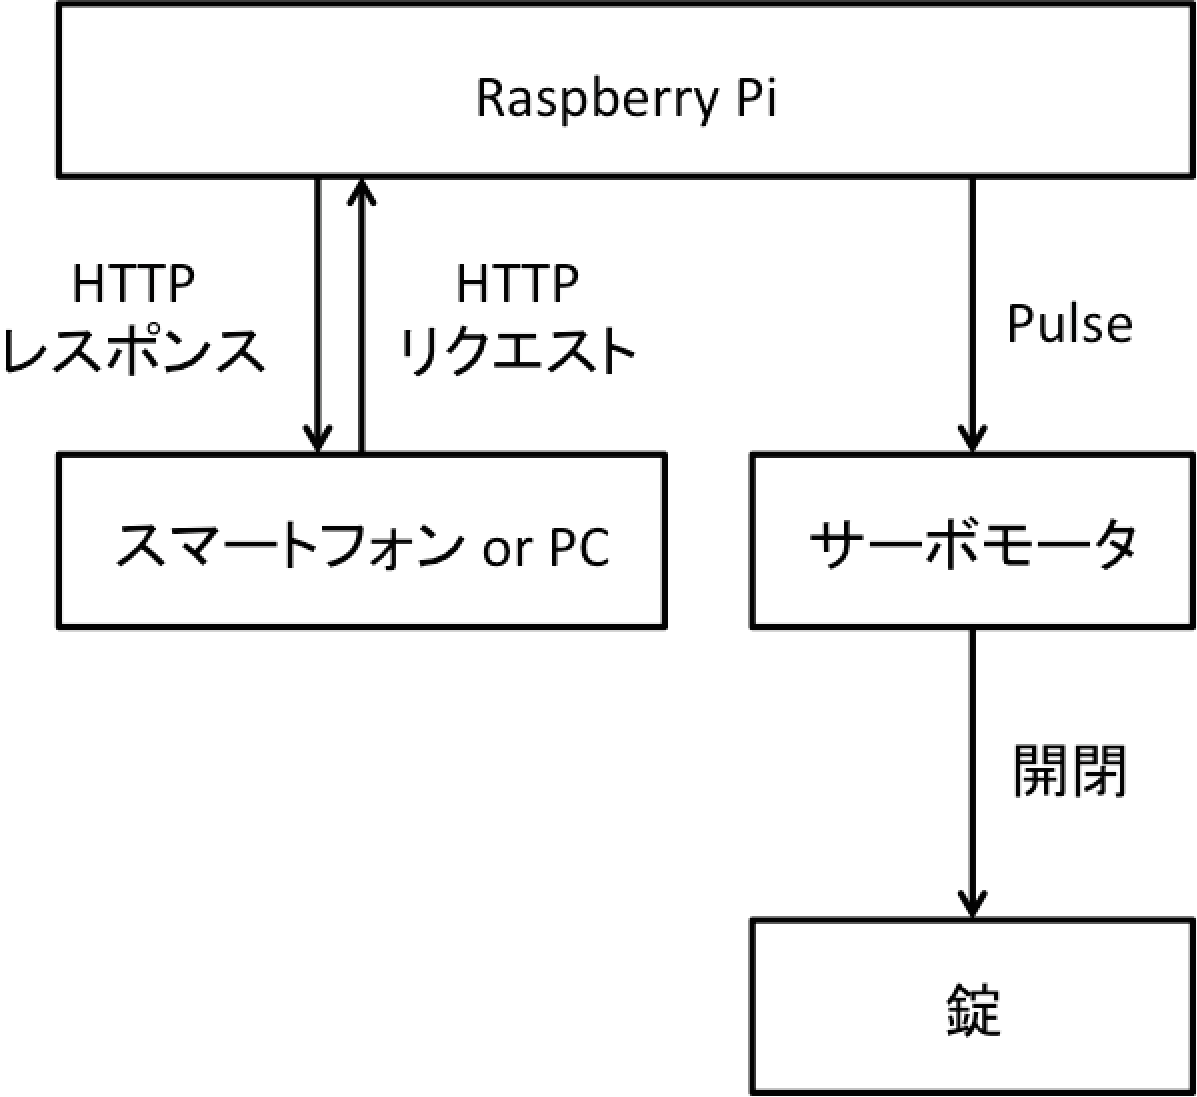
\includegraphics[width=0.35\textwidth]{./assets/system_fig.eps}
  \caption{システム図}
  \label{fig:system_fig}
\end{figure}

\subsection{モーター}
モーターはピンの消費が少なく外部電源の必要ないサーボモータを利用した.
サーボモータは図~\ref{fig:servo}, 表~\ref{tbl:servo_specifications}
のような仕様のものを利用し,
解錠に必要なトルクとスピードを満たすものを選択した.

\begin{figure}[htbp]
  \centering
  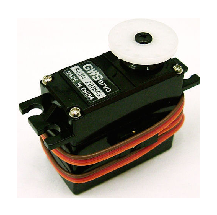
\includegraphics[width=0.2\textwidth]{./assets/servo.eps}
  \caption{サーボモータ}
  \label{fig:servo}
\end{figure}

\begin{table}[htbp]
  \begin{center}
    \begin{tabular}{cc}
      Torque & 3.4 kg (4.8V)  \\
      Weight & 64 g  \\
      Speed  & 0.23 sec / 60 deg (4.8V) \\
      Size   & 39.5 x 20 x 35.6 mm
    \end{tabular}
    \caption{GWSサーボ S03N/2BBMG/JRタイプ}
    \label{tbl:servo_specifications}
  \end{center}
\end{table}

\subsection{Webアプリケーション}
外部機器との通信において,モータの操作や鍵の共有
を行うためのインターフェースとしてWebアプリケーションを作成した.
作成したWebページは以下4ページである.

\begin{itemize}[noitemsep]
  \item ログインページ.(図~\ref{fig:login_page})
  \item 錠の状態,開閉操作ページ.(図~\ref{fig:control_page})
  \item ログ確認ページ.(図~\ref{fig:log_page})
  \item アクセス権付与ページ.(図~\ref{fig:authorize_page})
\end{itemize}

ログインは独自のアカウントは作成せず,Googleアカウントで行う.
Google APIを使ってメールアドレスや名前,プロフィール画像などが取得可能
であるため,基本情報などの入力なしにスムーズに利用へ
移ることができる.
共有はアクセス権のある者がメールアドレスを入力して与えるという形をとる.

また,錠の状態と開閉の操作ページ(図~\ref{fig:control_page})において,
多人数が利用することを考慮し,ブラウザの更新なしに開閉状態が
切り替わるようにした.
これはAjaxを用いて定期的にデータベース内の情報を取得することで実現した.

\begin{figure}[htbp]
  \begin{tabular}{cc}
    \begin{minipage}{0.5\hsize}
      \begin{center}
        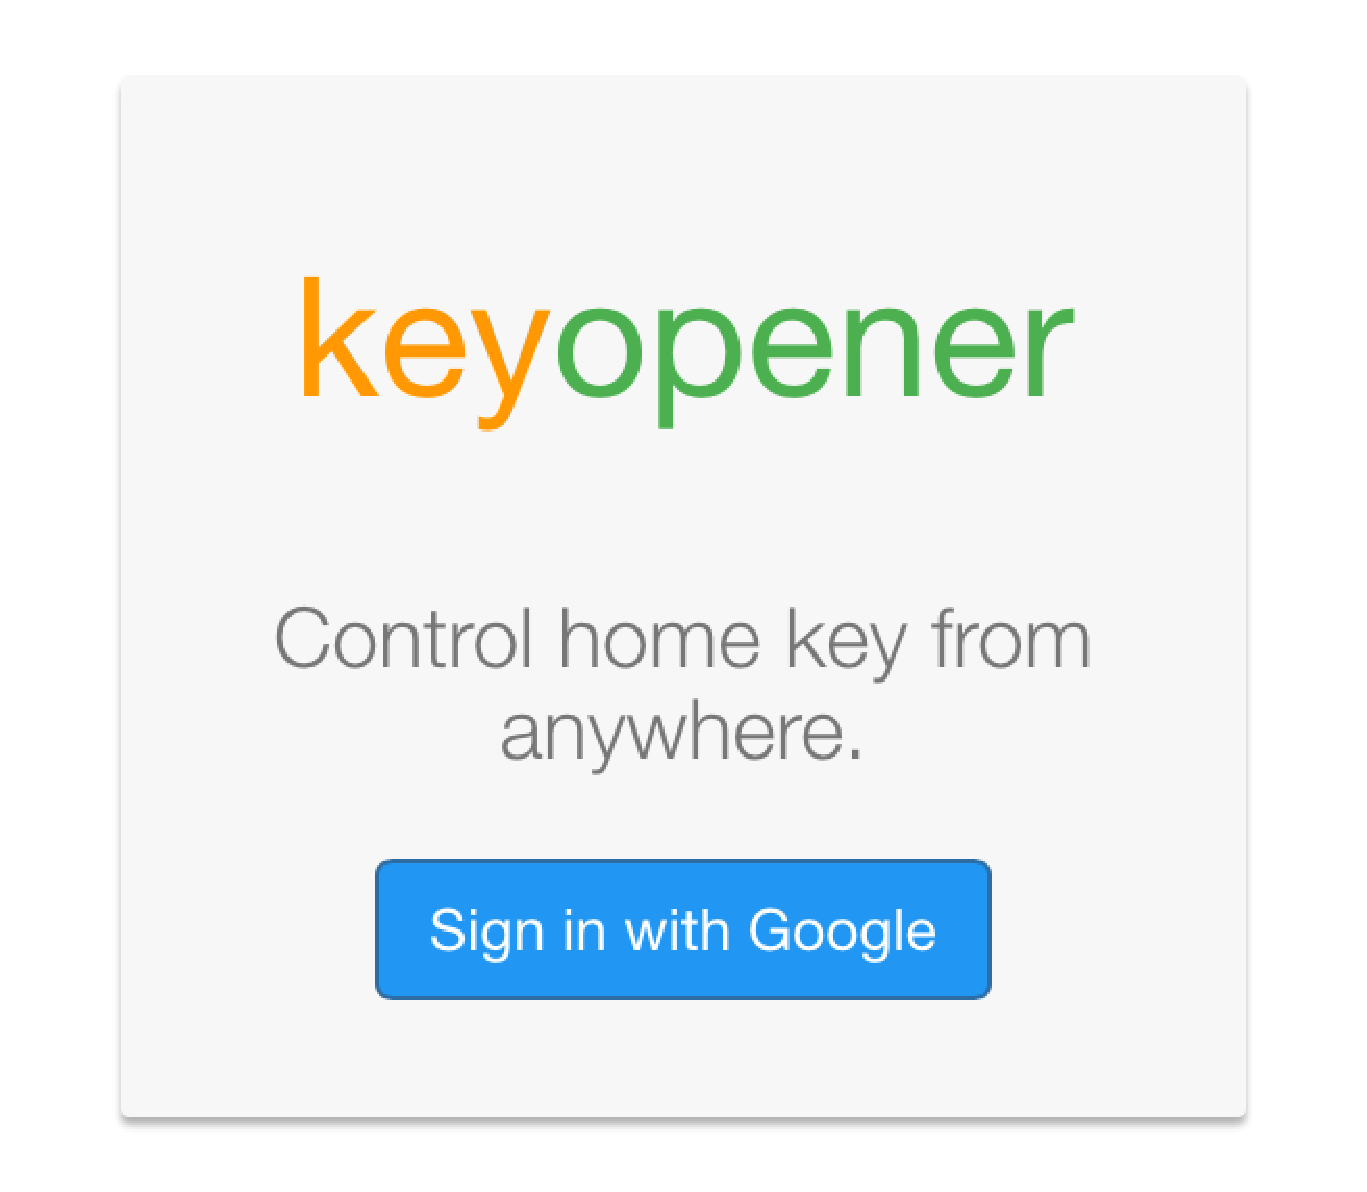
\includegraphics[width=0.8\textwidth]{./assets/login_page.eps}
        \caption{ログイン}
        \label{fig:login_page}
      \end{center}
    \end{minipage}
    \begin{minipage}{0.5\hsize}
      \begin{center}
        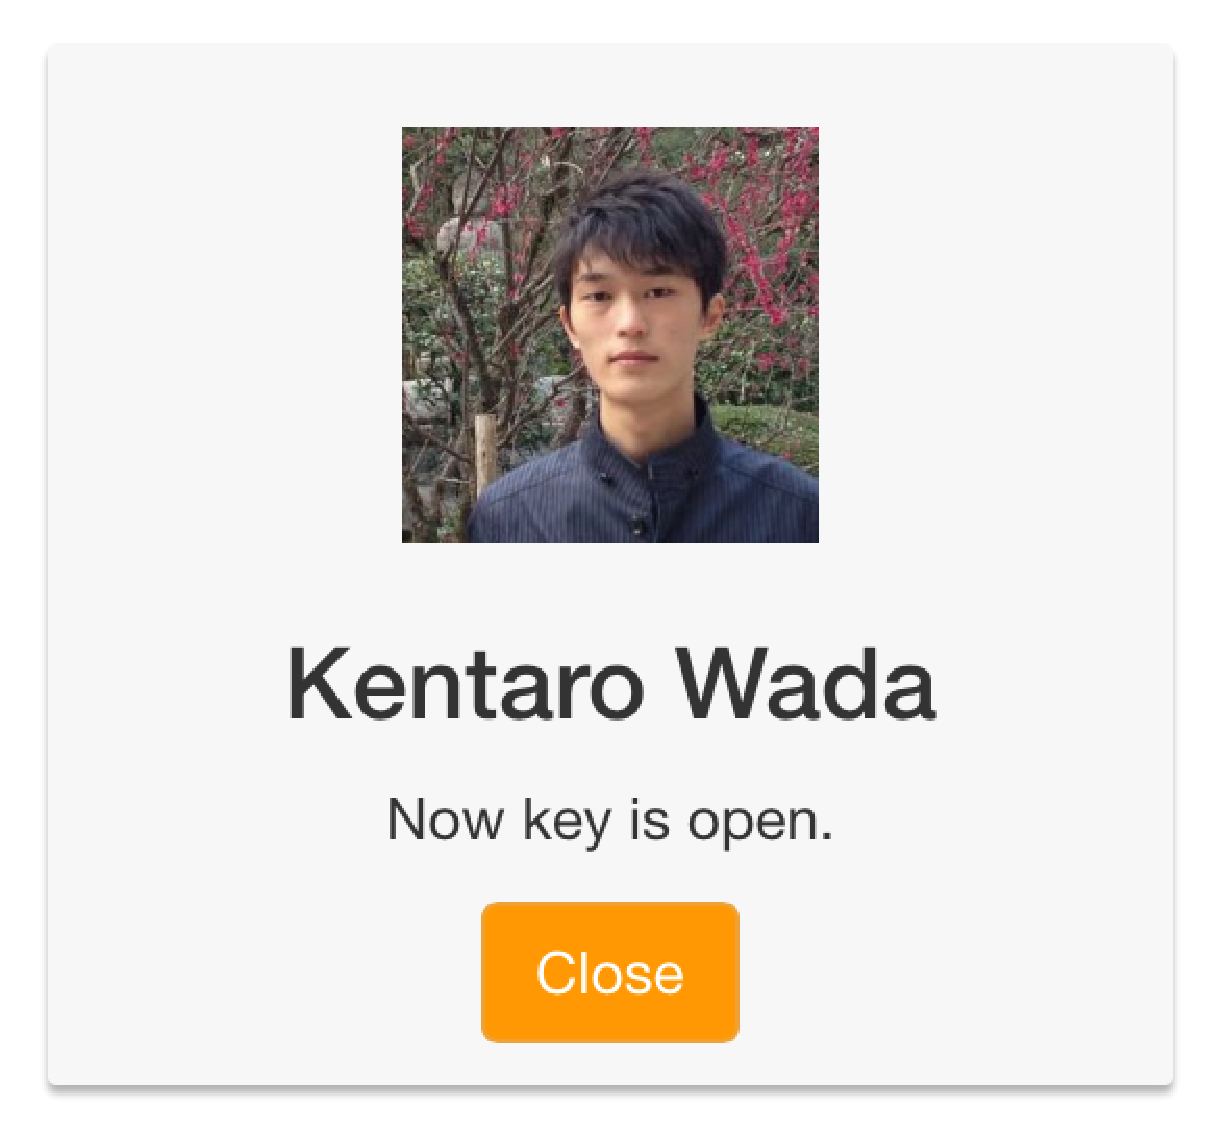
\includegraphics[width=0.75\textwidth]{./assets/control_page.eps}
        \caption{状態,開閉操作}
        \label{fig:control_page}
      \end{center}
    \end{minipage}
  \end{tabular}
\end{figure}

\begin{figure}[htbp]
  \begin{tabular}{cc}
    \begin{minipage}{0.5\hsize}
      \begin{center}
        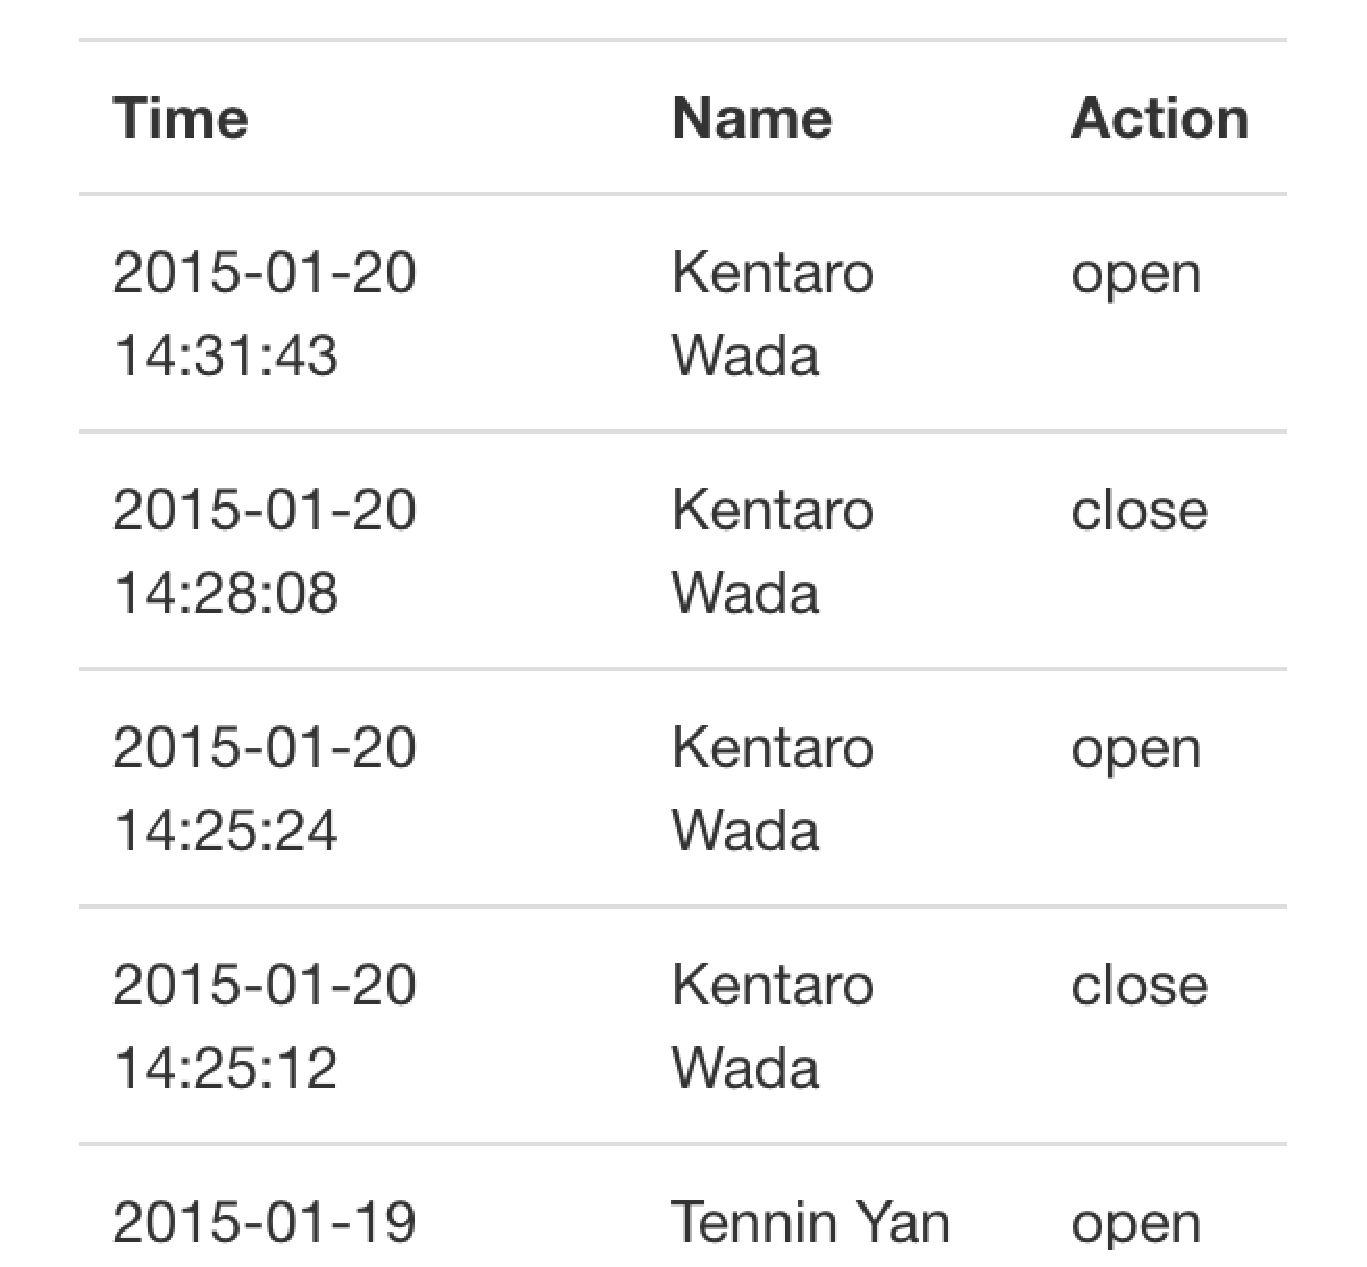
\includegraphics[width=0.7\textwidth]{./assets/log_page.eps}
        \caption{ログ確認}
        \label{fig:log_page}
      \end{center}
    \end{minipage}
    \begin{minipage}{0.5\hsize}
      \begin{center}
        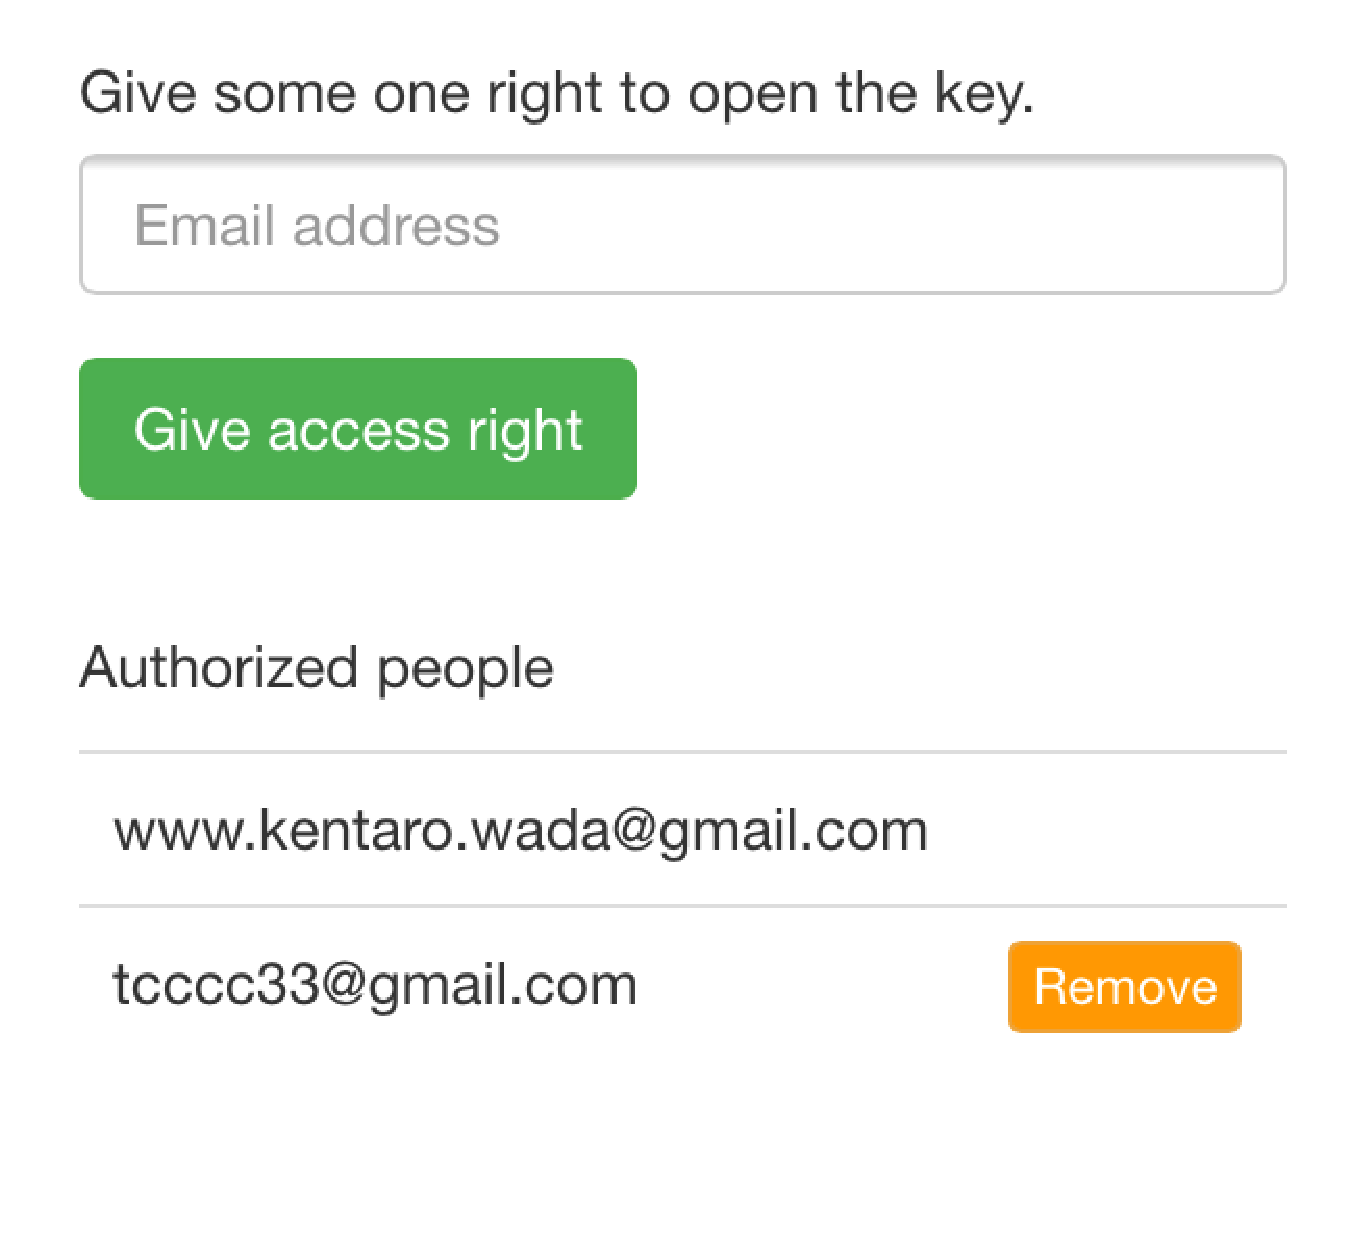
\includegraphics[width=0.7\textwidth]{./assets/authorize_page.eps}
        \caption{アクセス権付与}
        \label{fig:authorize_page}
      \end{center}
    \end{minipage}
  \end{tabular}
\end{figure}

\subsection{取付機構}
取付機構に関して,以下の点に留意した.

\begin{itemize}[noitemsep]
  \item 取り付けが容易であること.
  \item 不可逆な変形を伴わないこと.
  \item 多くのドアに対応できること.
\end{itemize}

機構は大きく図~\ref{fig:head},~\ref{fig:foot}
の二つからなっており,それぞれサムーンとドアノブに取り付ける.
サムターンとはドアの内側に付いている,錠の開閉に使う金具のことである.

サムターンへの取付部は,デバイスの自重を支えるためのものであり,
ネジで締めることでサムターンに固定される.
ドアノブ取付部は,モーター本体の回転を固定するためのもので,これによって
モーターの本体部は回転せず,サムターンに固定されている部分が回転し,
鍵が開くという仕組みである.

\begin{figure}[htbp]
  \begin{tabular}{cc}
    \begin{minipage}{0.5\hsize}
      \begin{center}
        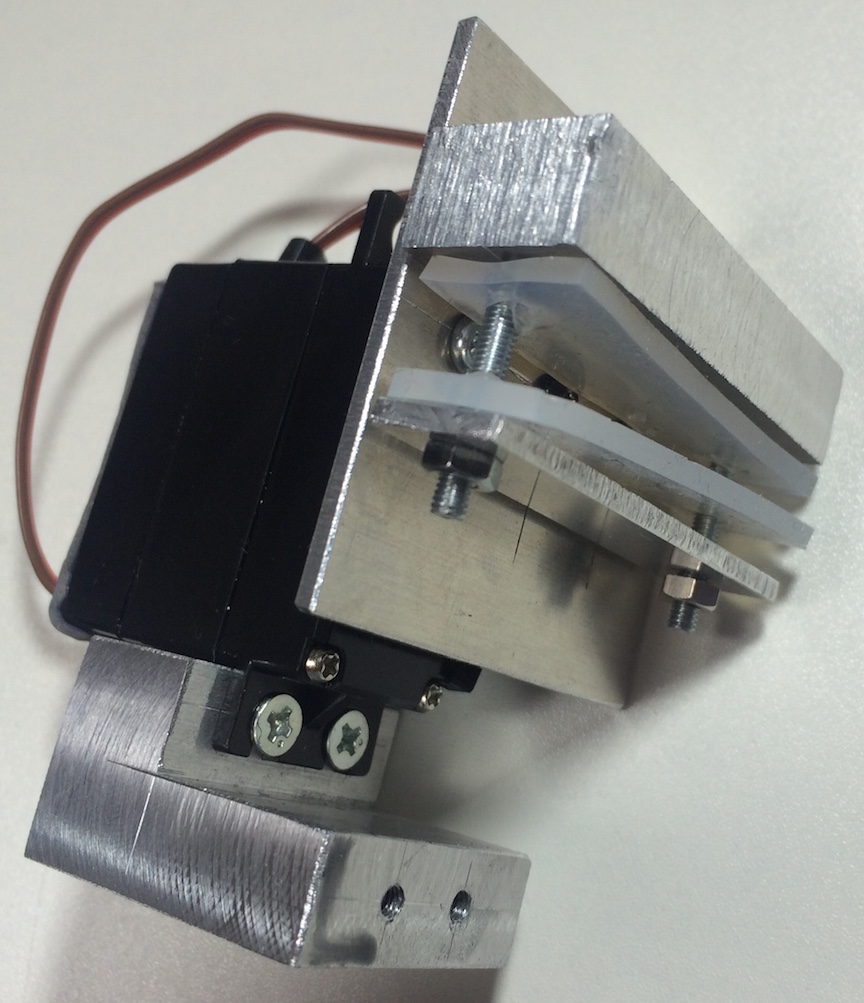
\includegraphics[width=0.6\textwidth]{./assets/head.eps}
        \caption{サムターン取付部}
        \label{fig:head}
      \end{center}
    \end{minipage}
    \begin{minipage}{0.5\hsize}
      \begin{center}
        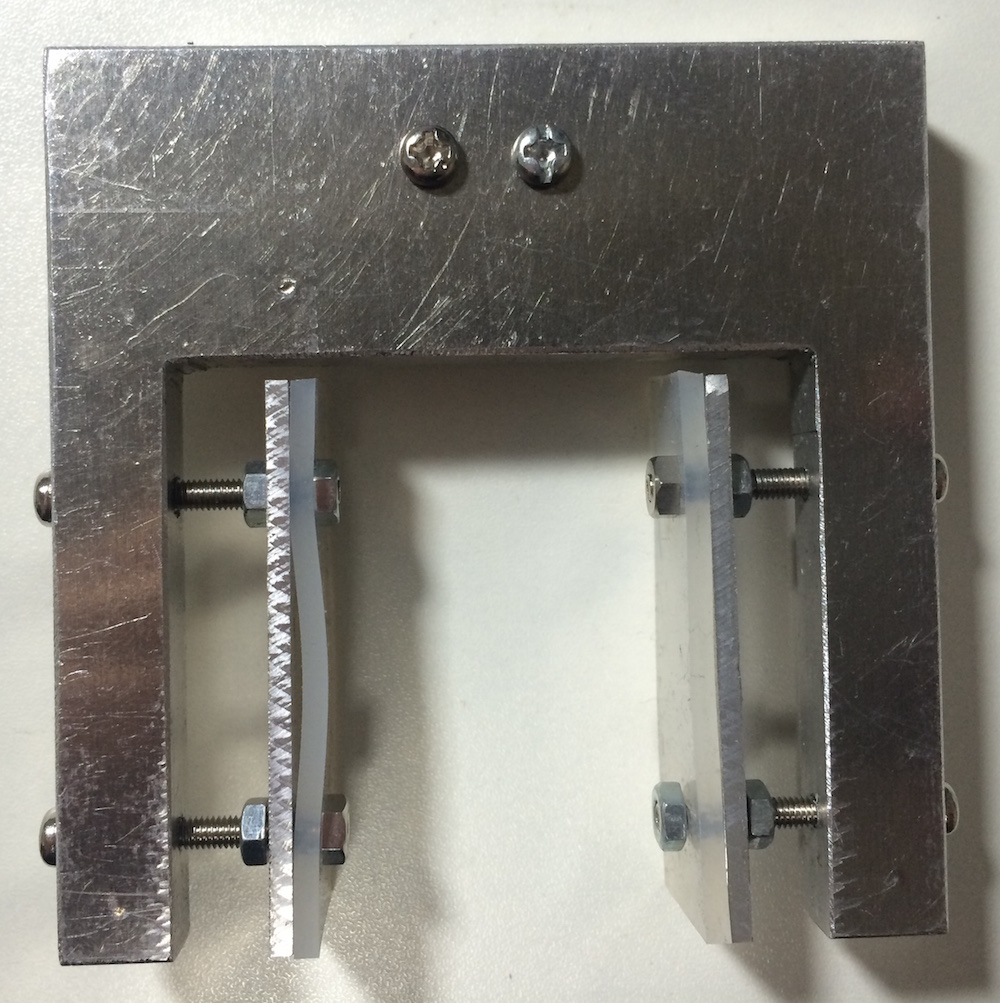
\includegraphics[width=0.7\textwidth]{./assets/foot.eps}
        \caption{ドアノブ取付部}
        \label{fig:foot}
      \end{center}
    \end{minipage}
  \end{tabular}
\end{figure}

\subsection{バッテリー}
バッテリーは図~\ref{fig:battery}, 表~\ref{tbl:battery}に示す,
モバイルバッテリーを採用した.

\begin{figure}[htbp]
  \centering
  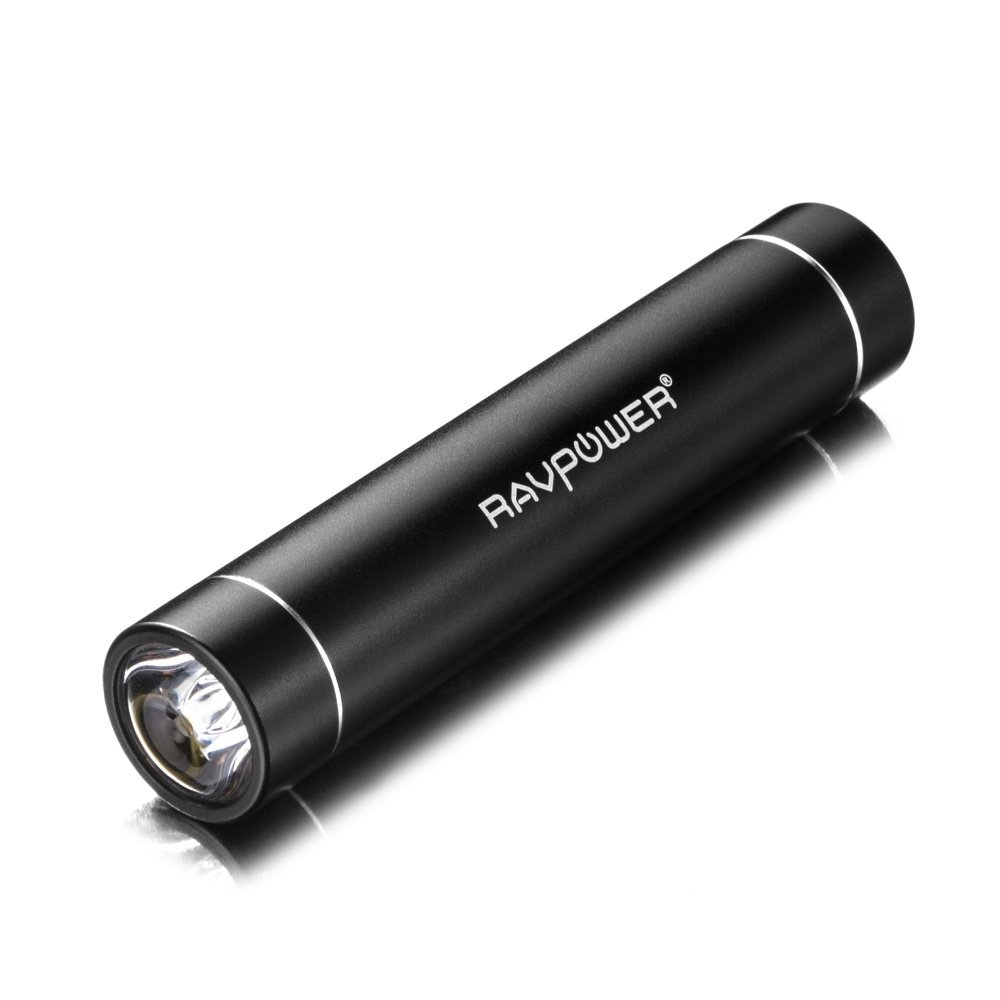
\includegraphics[width=0.2\textwidth]{./assets/battery.eps}
  \caption{バッテリー}
  \label{fig:battery}
\end{figure}

\begin{table}[htbp]
  \begin{center}
    \begin{tabular}{cc}
      Capacity & 3200 mAh \\
      Weight & 73 g \\
      Size & 108 x 22 x 22 mm \\
    \end{tabular}
    \caption{バッテリー仕様}
    \label{tbl:battery}
  \end{center}
\end{table}


\section{製作過程}
取付部の設計は,無侵襲で容易に取り外し可能な機構の実現のために
試作なども行ったため,時間を要した.

Webアプリケーションの開発は知識があったため,
それほど時間を必要とせず完了した.

調整期間には外部ネットワークからアクセスできるよう,
ネットワークルータの設定も行った.

\begin{itemize}[noitemsep]
  \item Raspberry Pi 設定. (2014/12/08)
  \item 取付部の設計. (2014/12/09-12, 15-19, 22, 2015/01/05-07)
  \item 取付部の加工. (2015/01/08-09, 01/13-16)
  \item Webアプリケーションの作成. (2015/01/17-18)
  \item 調整. (2015/01/19-22)
\end{itemize}


\section{動作結果}\label{sec:result}
最終的に組み立てたものが図~\ref{fig:complete}である.

\begin{figure}[htbp]
  \centering
  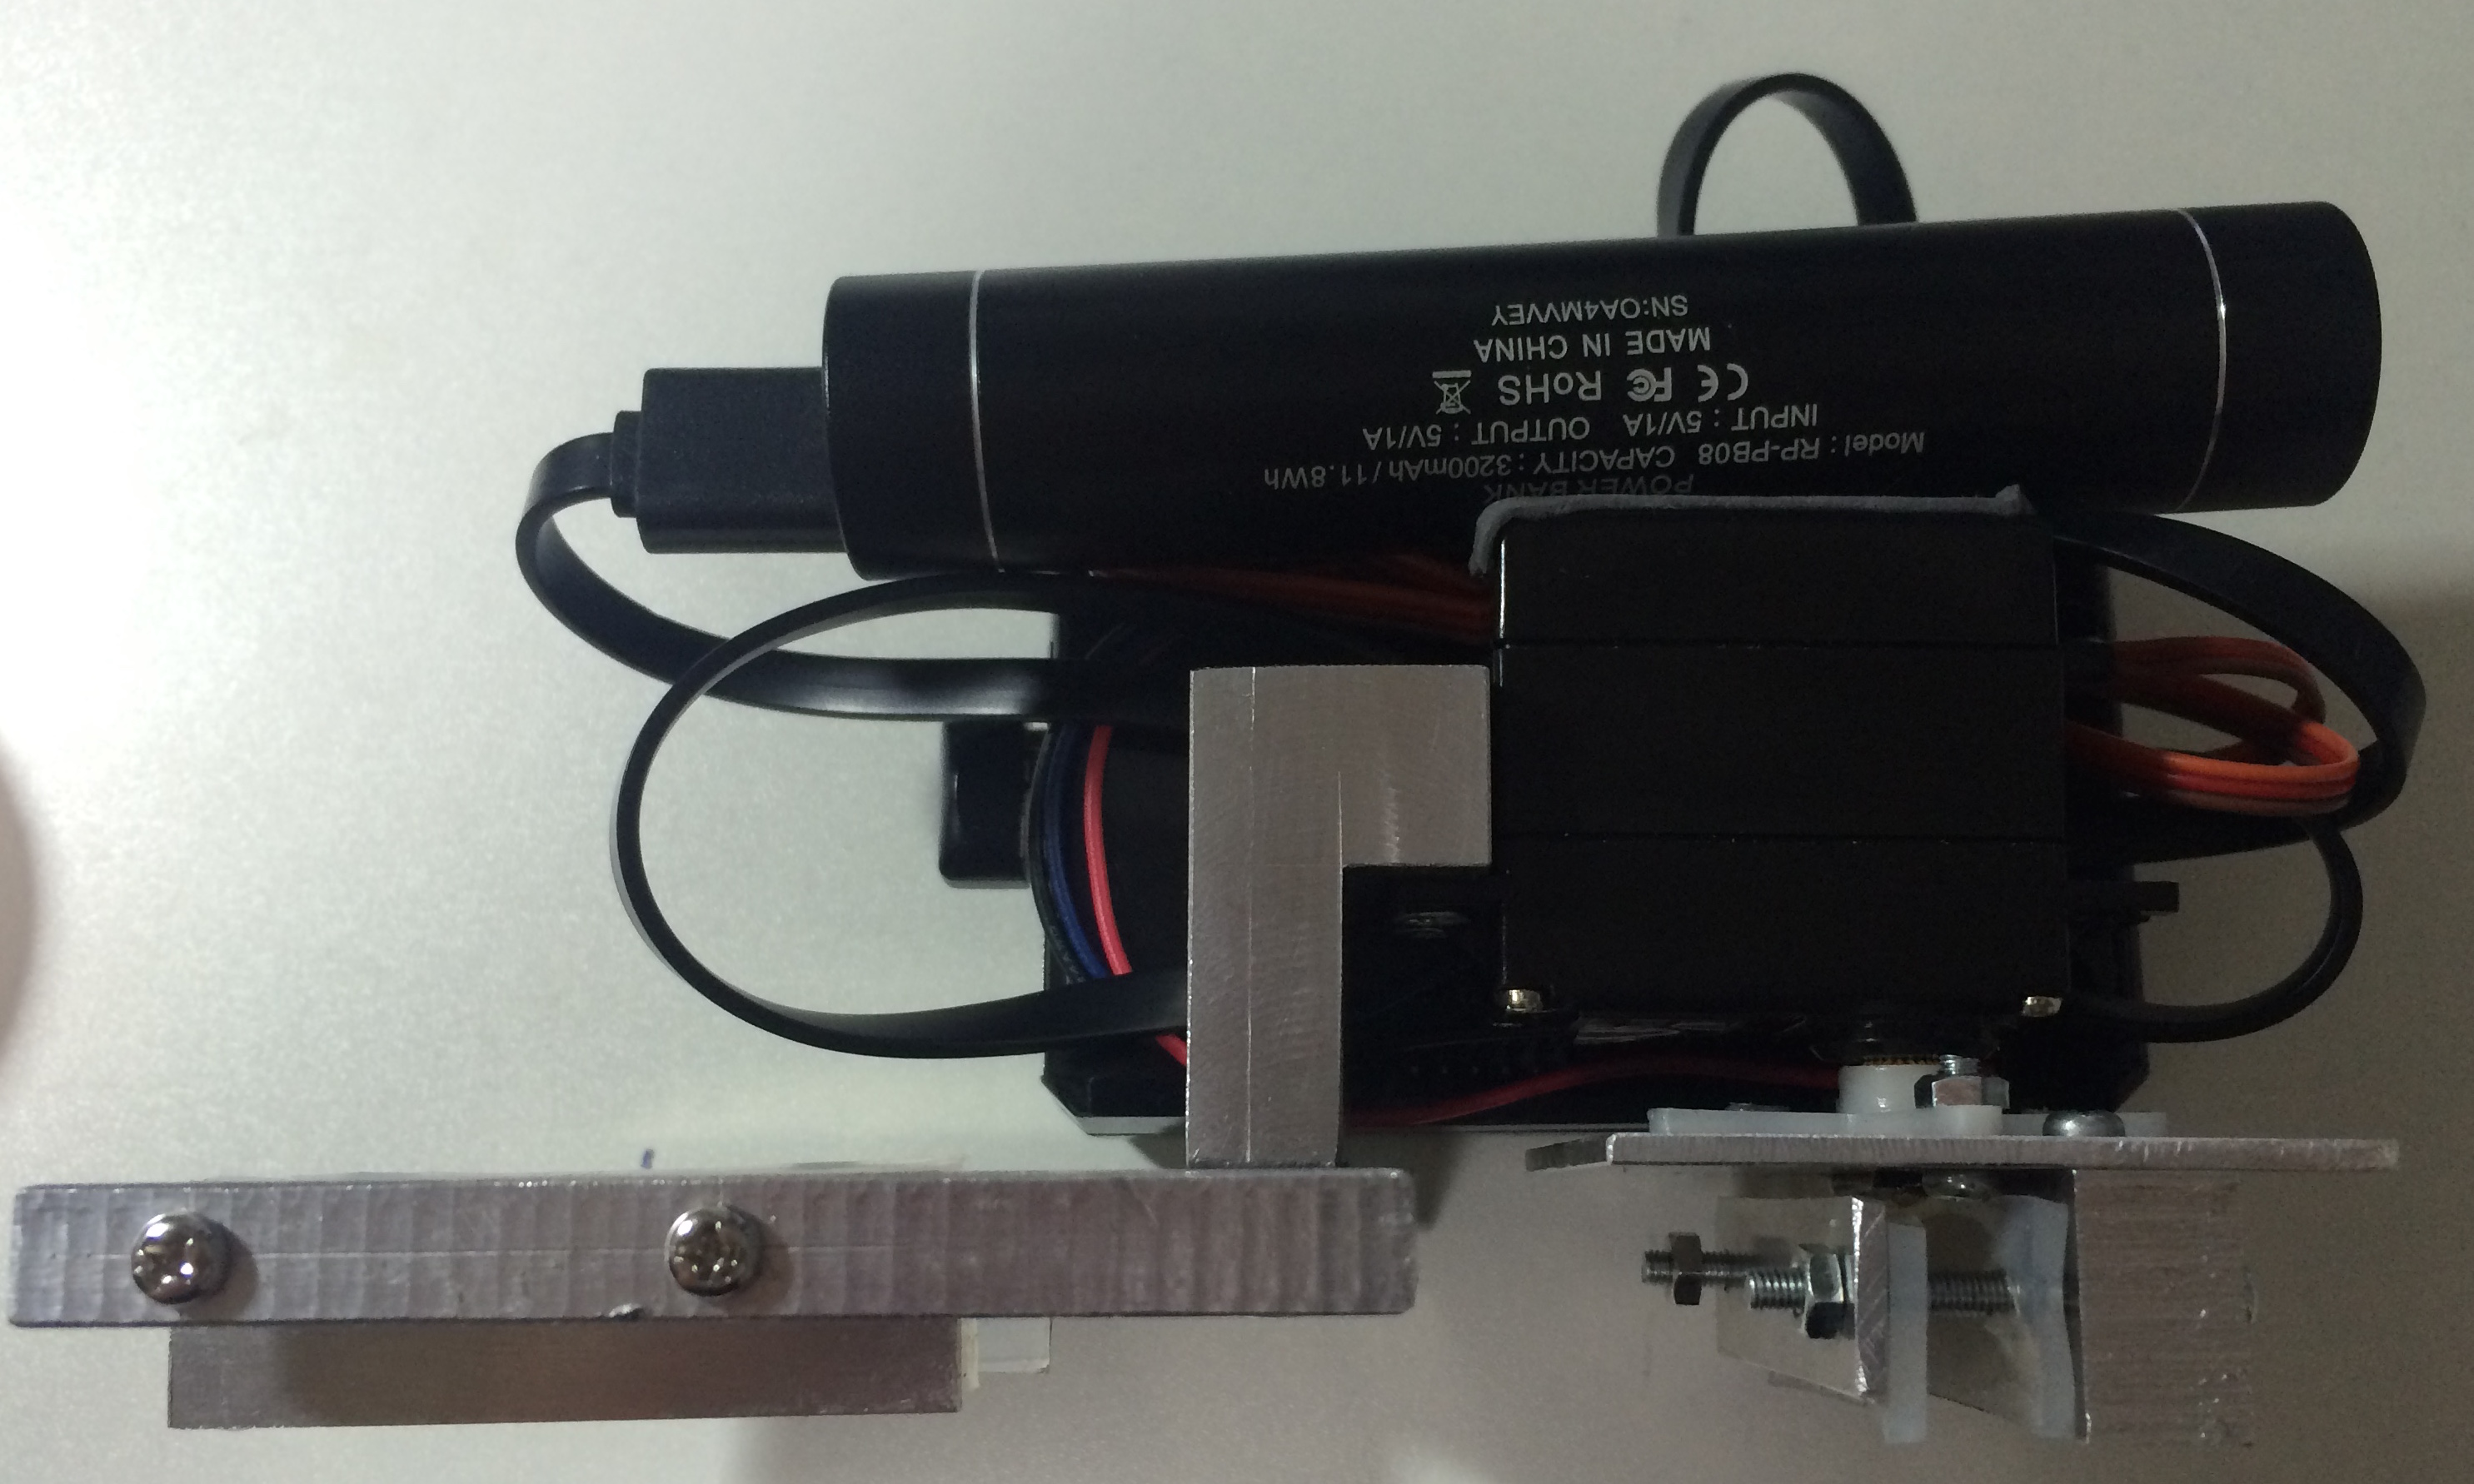
\includegraphics[width=0.35\textwidth]{./assets/complete.eps}
  \caption{ドア取り付け部分}
  \label{fig:complete}
\end{figure}

スマートフォンやPCのブラウザからアクセスし,ログイン,
アクセス権共有,ログ確認,鍵の開閉操作など問題なく動作した.

実際に取り付けを行うと,錠の中心軸とモータの軸とがずれている場合があるが,
一度回転を行うとモータのトルクによって位置調節が行われ,
二度目からは完全に軸が揃った状態になる.

電源に利用したモバイルバッテリーの連続稼働時間は24時間程度であった.


\section{考察}\label{sec:consideration}
鍵のオンライン化システムの有用性として,遠隔地からの錠の施錠確認,
多人数の共有スペースにおいて多数の鍵の擬似的生成など
が考えられ,今回の制作物も十分にその有用性を持っている.

課題としては,モバイルバッテリーの連続稼働時間が24時間と短いことから,
実際に利用する際はコンセントからの電源供給が必要になってしまうという
ものがある.これはモータを駆動するマイコンに電池消費の大きい
Raspberry Piを採用したことが一つの原因であると考えられ,
Webアプリケーションのためのサーバーを別で用意し,機能は制限されても
消費電力のより小さいマイコンを利用することが改善として必要だと言える.


\section{最後に}
自主プロジェクトで,実用的なIoTシステムを作りたいと考えていたので,
バッテリーの容量不足という問題で制限され,実用に耐えないものとなって
しまったことが悔しいが,プロジェクト期間中に一つ一つの課題を
解決していけたのは良い経験になったと思う.







\begin{thebibliography}{9}
  \bibitem{intro-iot} Cisco inSPire, 2013, http://cisco-inspire.jp/issues/0010/cover\_story.html
\end{thebibliography}


\end{document}

